\begin{appendices}

\chapter{Mockups de Interfaces del Sistema}
\label{anexo:Mockups}
---------------------------------------------------------------------------
\section{Perfil: Administración y Defensoría}
Este perfil integra las herramientas de gestión interna de la plataforma. El acceso está restringido al personal de la Defensoría de los Derechos Politécnicos y se divide en cuatro departamentos operativos con facultades diferenciadas para garantizar la debida atención de los expedientes.

% --- VISTA ADMINISTRATIVA 01 ---
\begin{figure}[h]
\centering
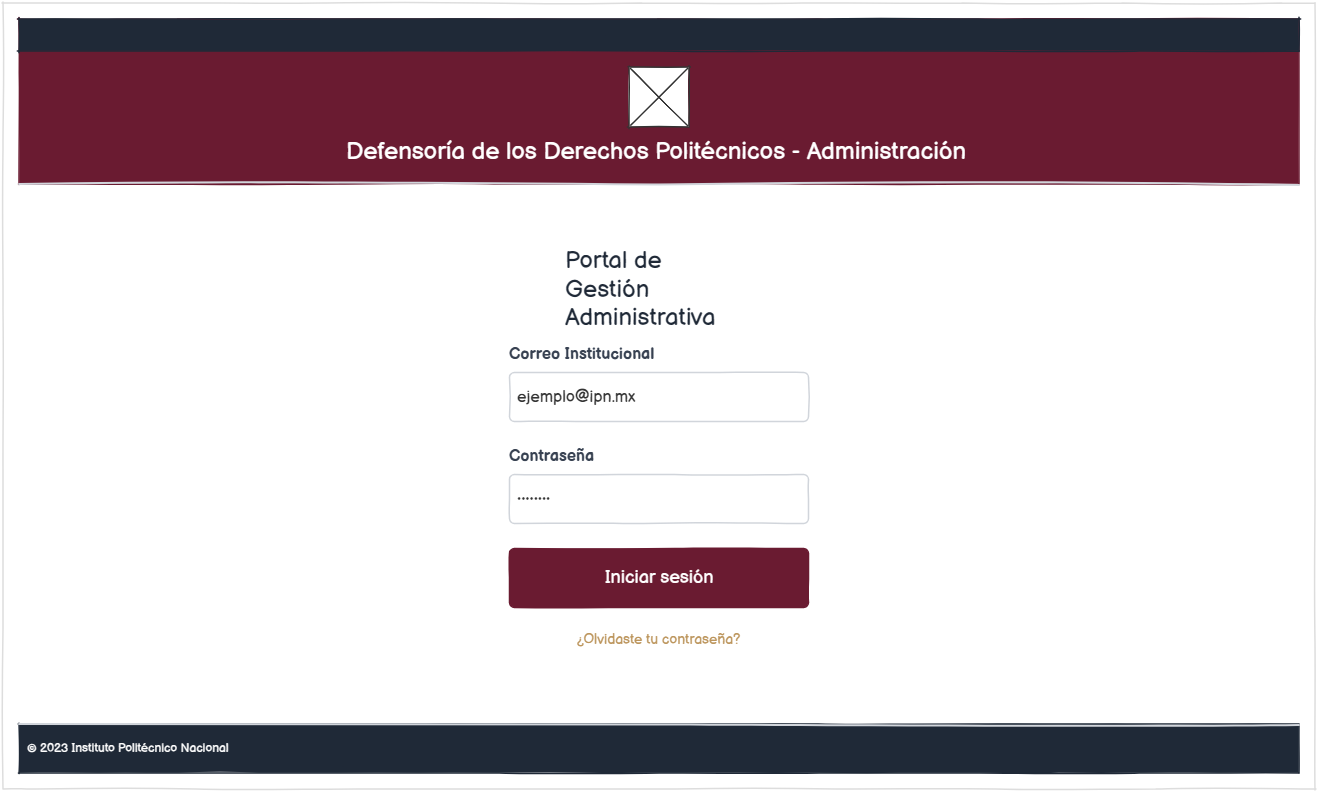
\includegraphics[width=0.65\textwidth]{imagenes/recepcion/InicioSesión_DDP.png}
\caption{MA-01: Portal de acceso al Sistema de Gestión Administrativa.}
\label{fig:ma01_login_adm}
\end{figure}

\noindent \textbf{Descripción de la interfaz (MA-01):} \
Esta interfaz representa el punto de acceso unificado para el personal de la Defensoría de los Derechos Politécnicos. A diferencia del portal ciudadano, esta vista está optimizada para la seguridad interna mediante un encabezado de administración que identifica claramente el módulo para evitar confusiones. El sistema presenta campos de credenciales vinculados al directorio institucional y un pie de página oficial que refuerza el carácter normativo del portal, permitiendo un acceso seguro y restringido a las funciones de gestión.


\clearpage

% --- VISTA ADMINISTRATIVA 02 ---
\begin{figure}[h]
\centering
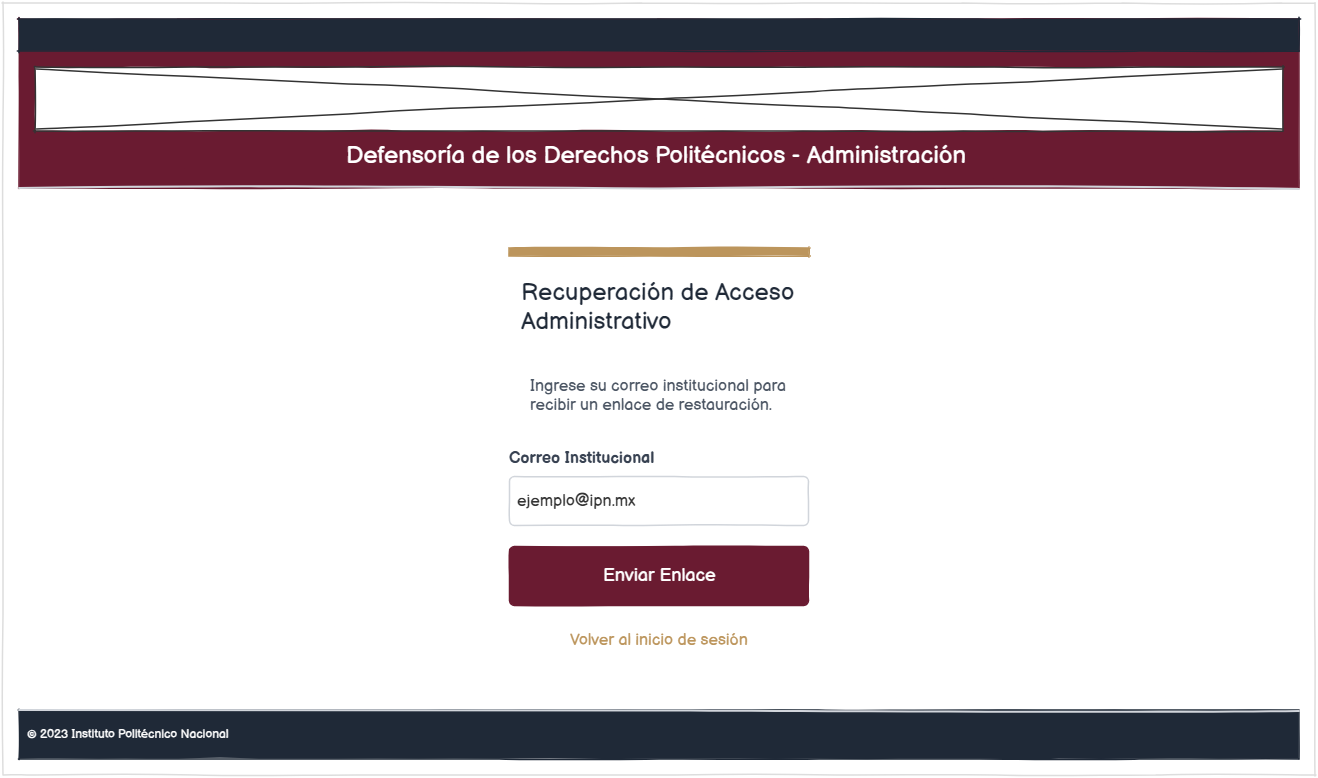
\includegraphics[width=0.65\textwidth]{imagenes/recepcion/RecuperaciónContraseñaDDP.png}
\caption{MA-02: Interfaz de recuperación de acceso para personal administrativo.}
\label{fig:ma02_recuperar_adm}
\end{figure}

\noindent \textbf{Descripción de la interfaz (MA-02):} \
Esta vista permite al personal de los cuatro departamentos restablecer sus credenciales de acceso de manera autónoma y segura. La validación institucional requiere exclusivamente el correo oficial para procesar la solicitud, asegurando que el enlace de restauración no sea desviado a cuentas externas. El flujo de recuperación cuenta con instrucciones directas y un control de navegación para volver al inicio de sesión, facilitando la recuperación del acceso sin comprometer la integridad del sistema administrativo.

\clearpage

\subsection{Departamento de Recepción}
Es el primer filtro del sistema, encargado de la validación inicial de los datos de entrada y la asignación preliminar de folios o turnos.

\begin{figure}[h]
\centering
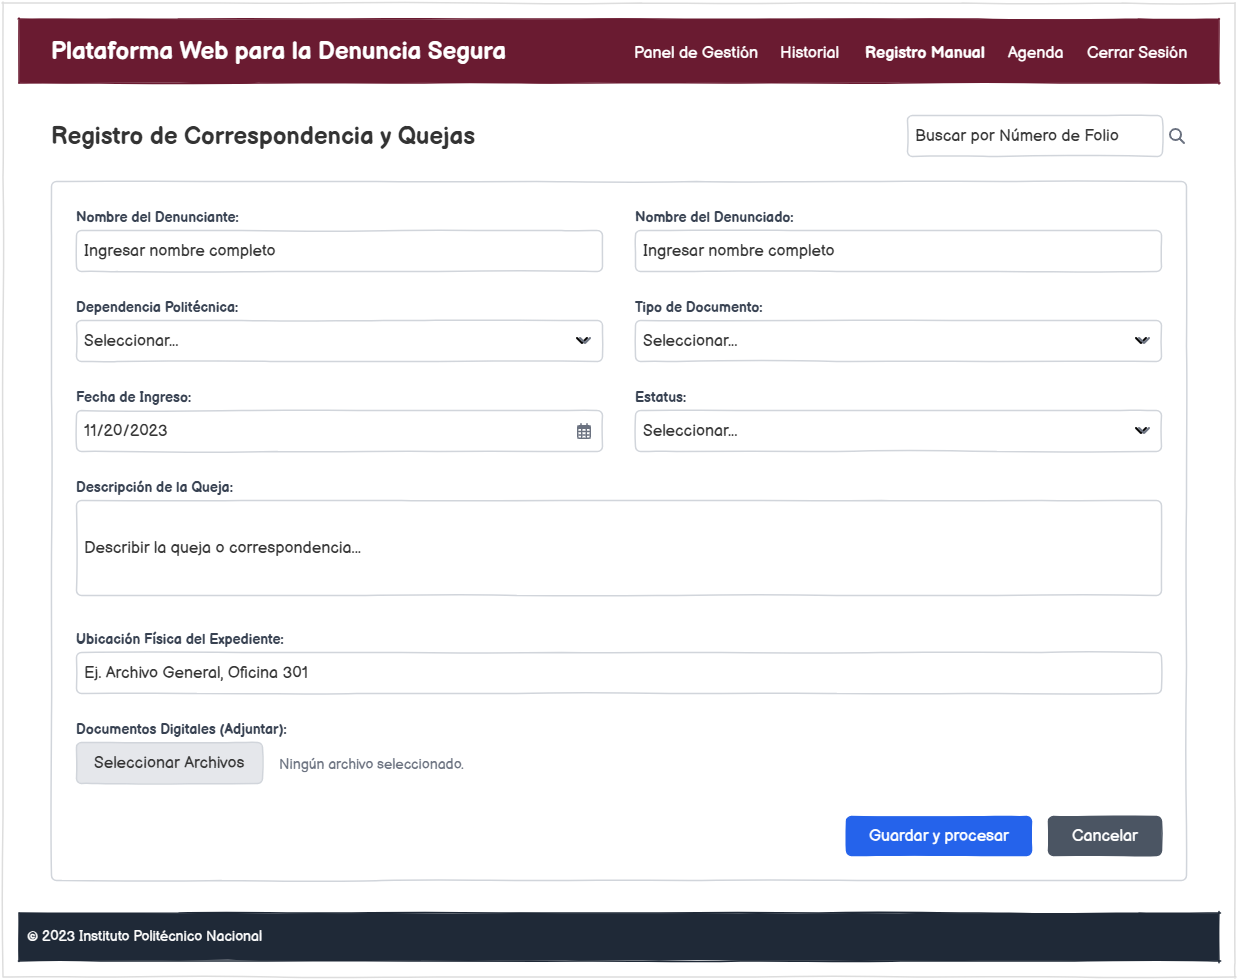
\includegraphics[width=0.65\textwidth]{imagenes/recepcion/RegistroManualQueja.png}
\caption{MA-03: Formulario de registro manual de correspondencia y quejas.}
\label{fig:ma03_registro_manual}
\end{figure}

\noindent \textbf{Descripción de la interfaz (MA-03):} \
Esta interfaz permite al personal administrativo registrar quejas o correspondencia recibida de manera presencial, facilitando la creación de un gemelo digital del expediente físico. La pantalla integra un buscador de folio para evitar duplicidad, campos para los datos de los sujetos involucrados y selectores para la clasificación administrativa y el estatus. Un elemento crítico es el campo especializado para registrar la ubicación del archivo físico, lo que garantiza la trazabilidad entre el papel original y el repositorio digital mediante la carga de evidencias escaneadas.


\clearpage

% --- VISTA 04: PANEL DE GESTIÓN ---
\begin{figure}[h]
\centering
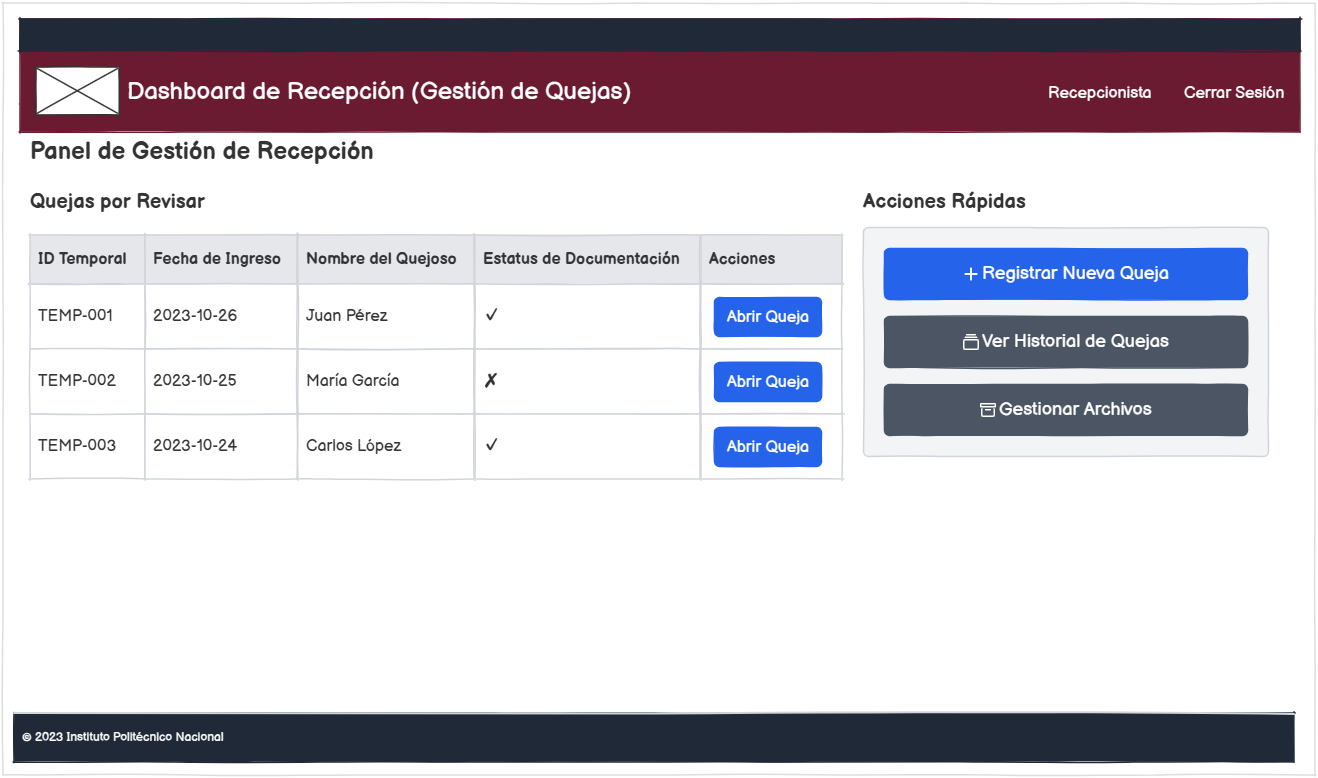
\includegraphics[width=0.65\textwidth]{imagenes/recepcion/PanelGestiónRecepción.png}
\caption{MA-04: Panel de gestión de recepción (Dashboard).}
\label{fig:ma04_dashboard_recepcion}
\end{figure}

\noindent \textbf{Descripción de la interfaz (MA-04):} \
Este tablero de control permite al personal de recepción monitorear las quejas entrantes de manera centralizada mediante una tabla operativa que utiliza identificadores temporales para registros pendientes de validación. La interfaz incluye indicadores visuales que señalan si un expediente cuenta con documentación completa, permitiendo el acceso directo al detalle de cada registro. Asimismo, un menú de acciones rápidas facilita tareas como el registro de nuevas quejas o la consulta del historial, manteniendo siempre visible el rol de recepcionista para asegurar la consistencia de los permisos.

\vspace{1cm}

% --- VISTA 05: VALIDACIÓN DE REQUISITOS ---
\begin{figure}[h]
\centering
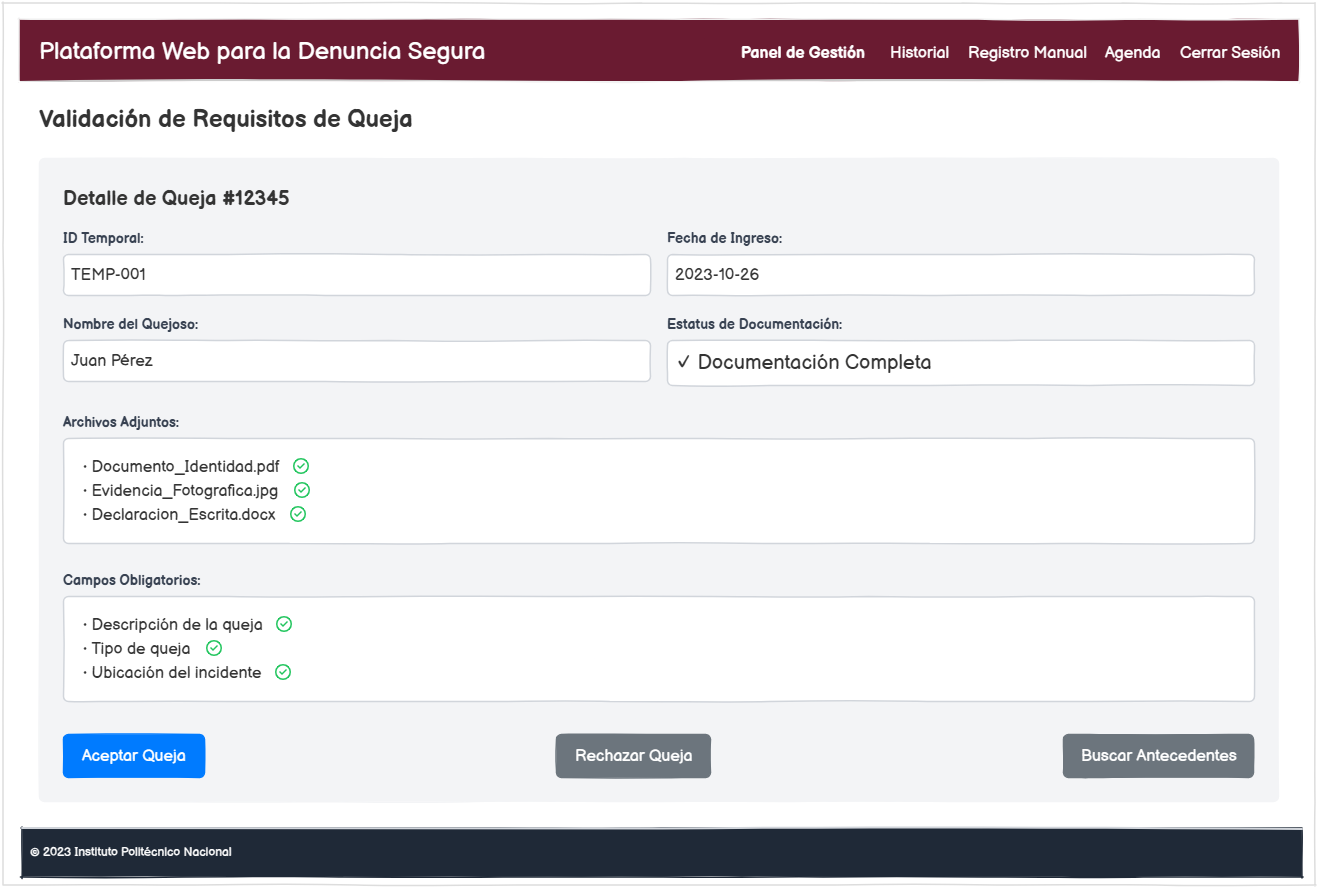
\includegraphics[width=0.65\textwidth]{imagenes/recepcion/ValidaciónRequisitosQueja.png}
\caption{MA-05: Módulo de validación de requisitos de queja.}
\label{fig:ma05_validacion_requisitos}
\end{figure}

\noindent \textbf{Descripción de la interfaz (MA-05):} \
Esta interfaz constituye el control de calidad del sistema, donde el personal asegura que cada solicitud cumpla con los estándares normativos. Presenta un resumen del expediente y un listado detallado de archivos adjuntos validados mediante iconos de verificación. El sistema obliga a la revisión de campos obligatorios como la descripción y la ubicación del incidente, concluyendo el proceso con botones de control que permiten aceptar la queja para su formalización, rechazarla por inconsistencias o realizar una búsqueda exhaustiva de antecedentes antes de su envío.

\vspace{1cm}

% --- VISTA 06: NOTIFICACIÓN DE RECHAZO ---
\begin{figure}[h]
\centering
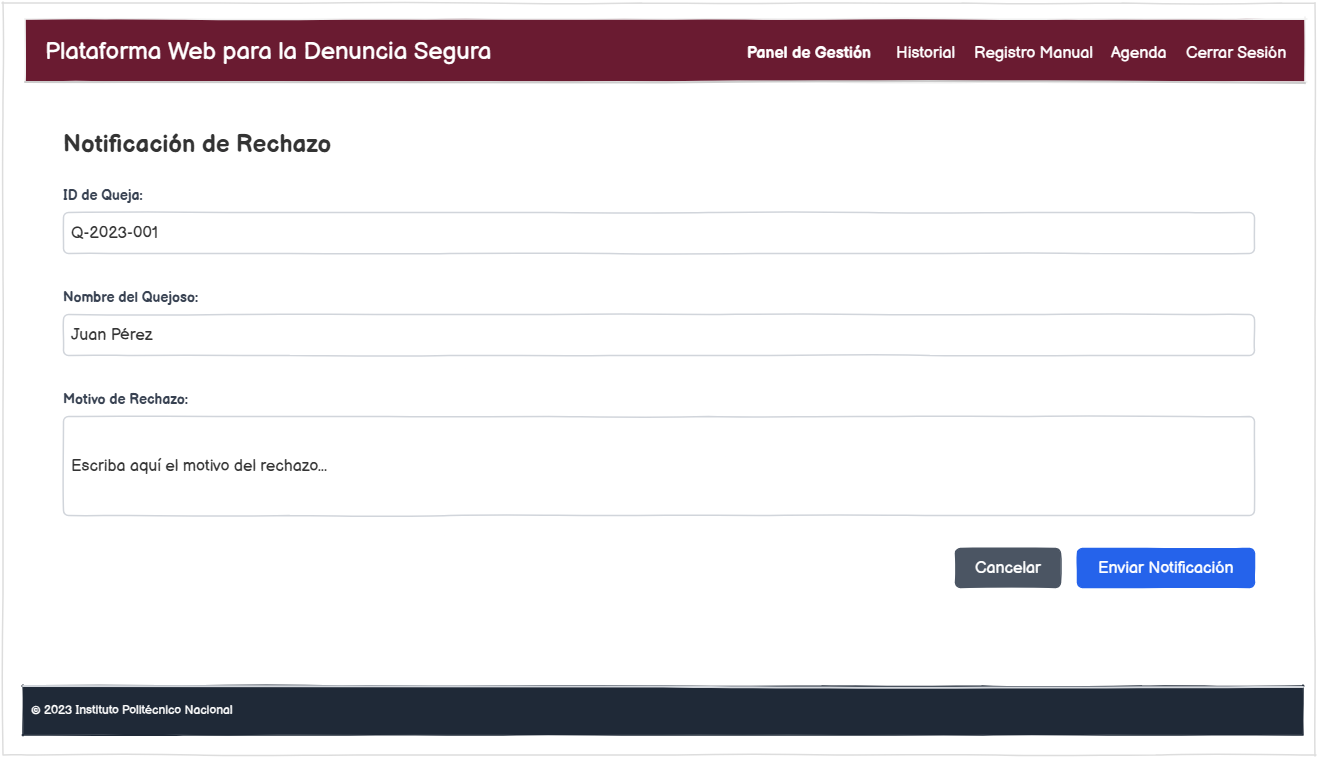
\includegraphics[width=0.65\textwidth]{imagenes/recepcion/NotificacionRechazo.png}
\caption{MA-06: Interfaz de notificación de rechazo por incumplimiento.}
\label{fig:ma06_notificacion_rechazo}
\end{figure}

\noindent \textbf{Descripción de la interfaz (MA-06):} \
Esta pantalla se activa al determinar que una solicitud no cumple con los requisitos mínimos, permitiendo informar al quejoso de manera formal sobre las deficiencias detectadas. La interfaz vincula automáticamente el ID del trámite y el nombre del usuario, ofreciendo un área de texto libre para que el administrativo redacte el motivo técnico o jurídico del rechazo. Una vez procesada la notificación, el sistema dispara un correo automático, permitiendo al personal retornar a sus labores mediante un menú de navegación persistente que conecta con la agenda e historial.

\vspace{1cm}

% --- VISTA 07: ANTECEDENTES Y CANALIZACIÓN ---
\begin{figure}[h]
\centering
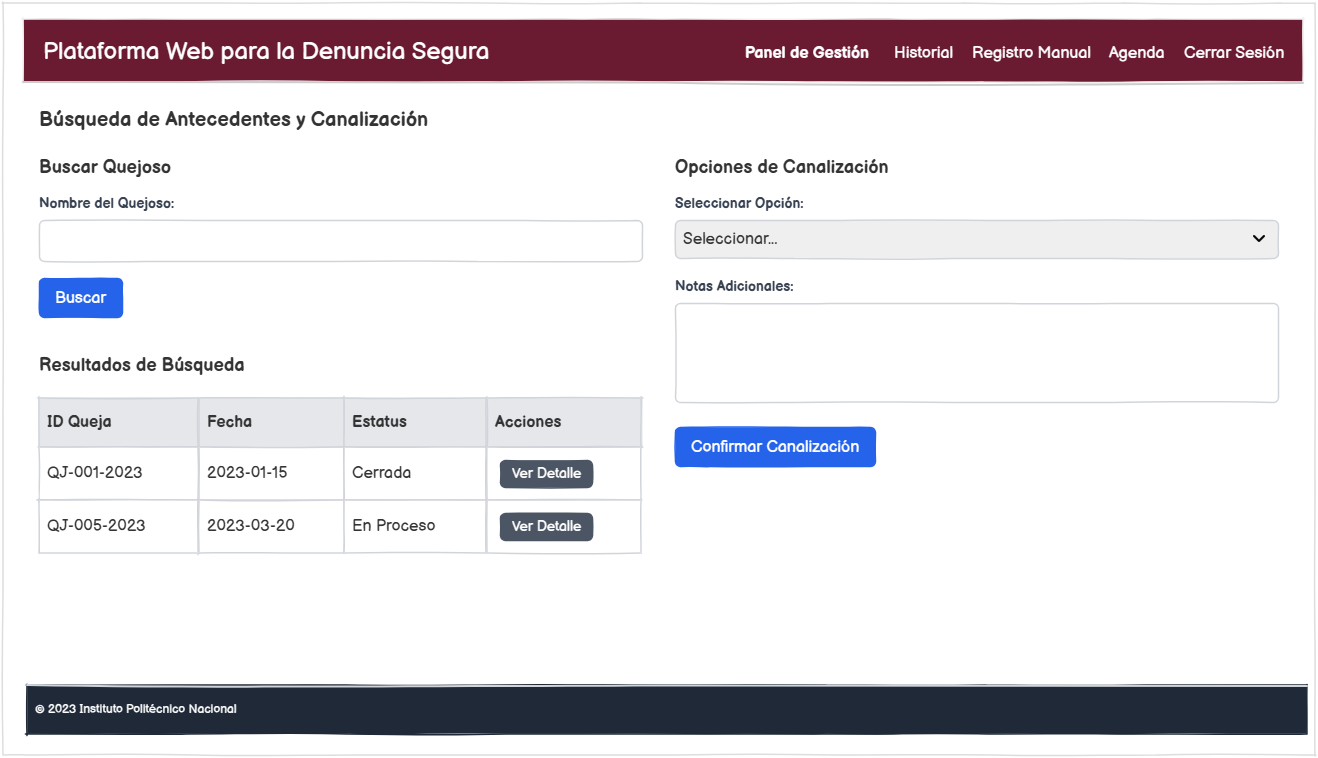
\includegraphics[width=0.65\textwidth]{imagenes/recepcion/BuesquedaAntecedentesCanalizacion.png}
\caption{MA-07: Módulo de búsqueda de antecedentes y canalización interna.}
\label{fig:ma07_canalizacion}
\end{figure}

\noindent \textbf{Descripción de la interfaz (MA-07):} \
Esta pantalla representa el último paso operativo en el área de Recepción, funcionando como motor de búsqueda y herramienta de traslado de expedientes. El sistema permite identificar procesos previos del quejoso para evitar duplicidades, mostrando una tabla de resultados con el historial de trámites anteriores. Para finalizar, el administrativo utiliza el panel de canalización para seleccionar el departamento de destino, agregando notas adicionales que orienten al siguiente analista antes de confirmar el envío y actualizar el estatus global del trámite.

\subsection{Departamento de Primer Contacto}
Este departamento se encarga de la atención personalizada al quejoso. Su función principal es realizar la entrevista inicial, analizar la naturaleza de la queja y determinar si el asunto es competencia de la Defensoría o si debe ser orientado a otra instancia.

% --- VISTA 08: BANDEJA DE ANÁLISIS ---
\begin{figure}[h]
\centering
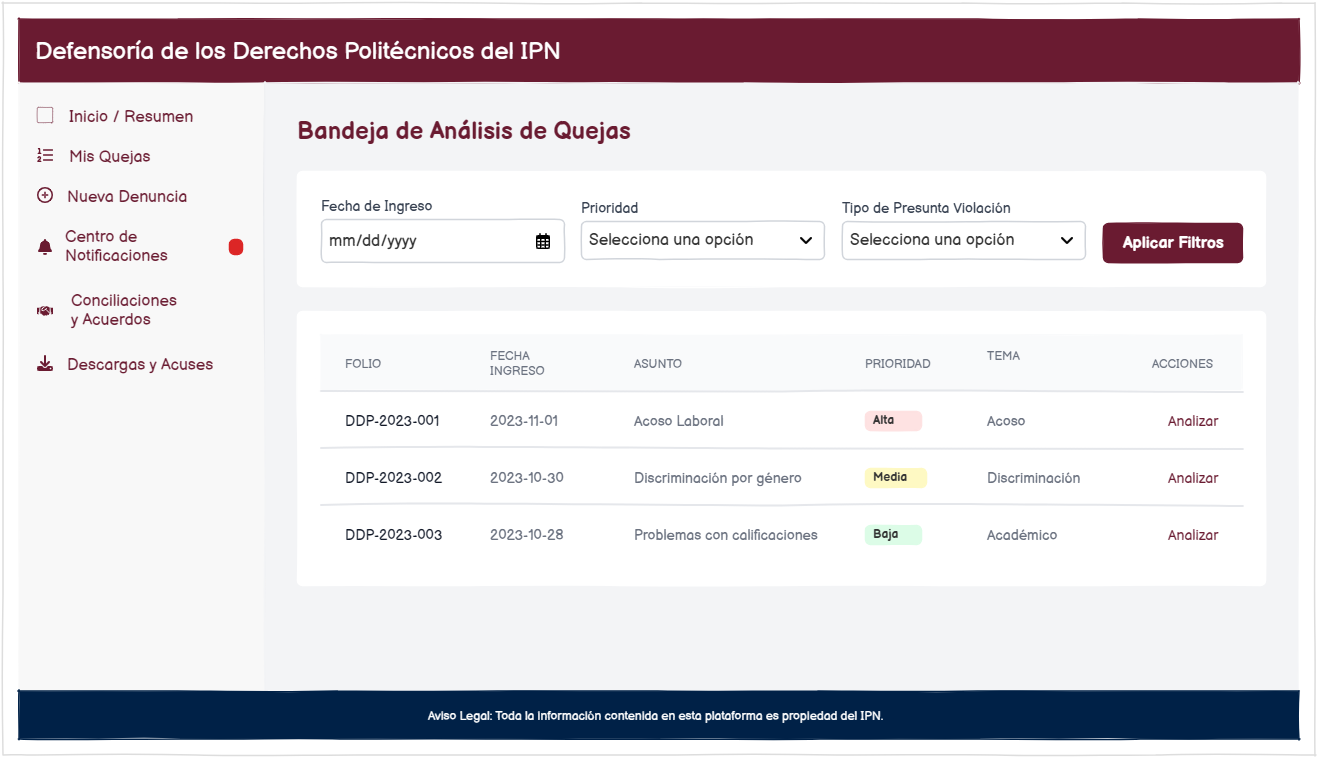
\includegraphics[width=0.65\textwidth]{imagenes/primercontacto/DashboardoAnalisisQuejas.png}
\caption{MA-08: Bandeja de análisis de quejas para Primer Contacto.}
\label{fig:ma08_analisis_dashboard}
\end{figure}

\noindent \textbf{Descripción de la interfaz (MA-08):} \
Esta interfaz constituye la herramienta principal del abogado o analista de Primer Contacto, diseñada para organizar de manera eficiente las quejas canalizadas desde el área de Recepción. La pantalla integra un módulo de filtrado avanzado que permite segmentar la carga de trabajo por fecha, prioridad y tipo de violación, facilitando la identificación de casos urgentes. A través de una tabla de gestión operativa, el personal puede visualizar los folios oficiales y los temas asignados, utilizando un sistema visual de etiquetas de colores para jerarquizar los hechos reportados. Finalmente, el control de análisis permite al funcionario acceder al detalle del expediente para iniciar formalmente la calificación jurídica.

\vspace{1cm}

\begin{figure}[h]
\centering
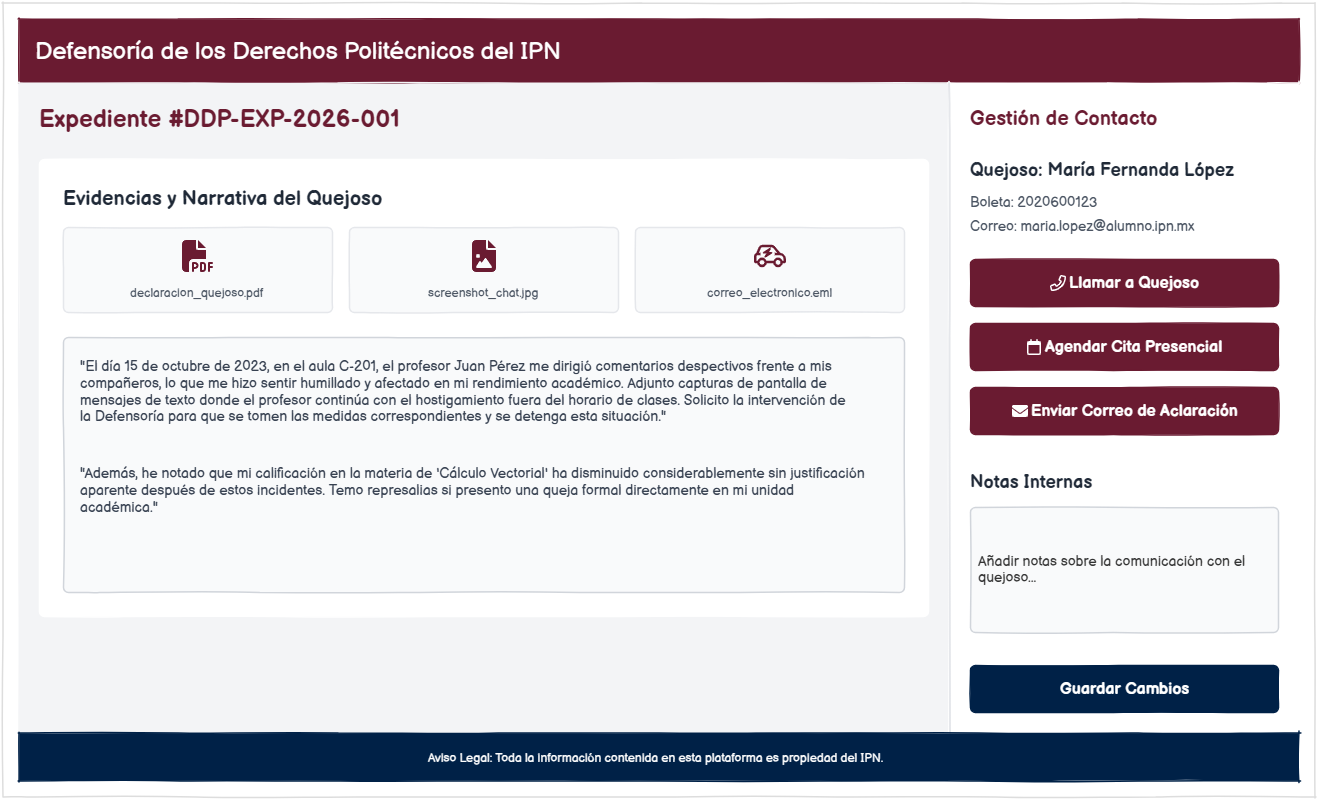
\includegraphics[width=0.65\textwidth]{imagenes/primercontacto/AnalisisExpediente.png}
\caption{MA-09: Interfaz de estudio de narrativa y evidencias.}
\label{fig:ma09_analisis_expediente}
\end{figure}

\noindent \textbf{Descripción de la interfaz (MQ-09):} \
Esta pantalla centraliza toda la información aportada por el quejoso para facilitar una evaluación legal exhaustiva por parte del analista. La interfaz dispone de un visor de evidencias con iconos diferenciados por formato, permitiendo una rápida revisión de los archivos adjuntos, junto a un área dedicada a la narrativa de los hechos para identificar presuntas violaciones de derechos. Además, se integra un panel de gestión de contacto con herramientas de comunicación inmediata para agendar citas o solicitar aclaraciones, complementado con una bitácora de notas internas donde el analista puede registrar observaciones técnicas que aseguren la continuidad del caso.

\clearpage


% --- VISTA 10: AGENDAR CITAS ---
\begin{figure}[h]
\centering
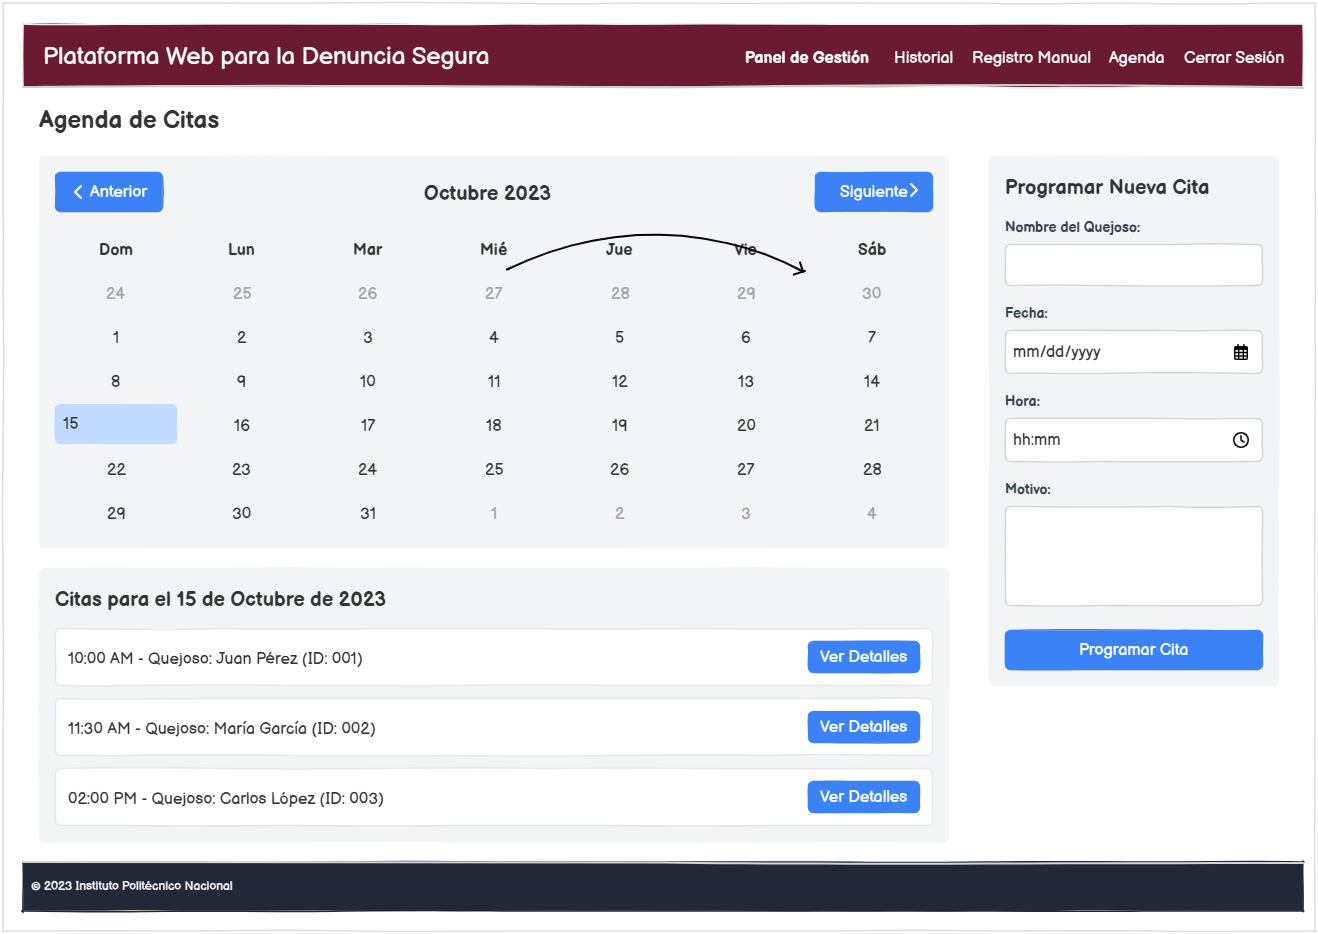
\includegraphics[width=0.65\textwidth]{imagenes/primercontacto/AgendarCitas.png}
\caption{MA-10: Módulo de agenda institucional para entrevistas de calificación.}
\label{fig:ma10_agenda_citas}
\end{figure}

\noindent \textbf{Descripción de la interfaz (MA-10):} \
Esta interfaz es fundamental para gestionar la interacción directa entre el analista y el quejoso, permitiendo organizar las diligencias necesarias para profundizar en los hechos. Presenta un calendario de disponibilidad dinámico que ayuda a evitar el traslape de horarios y optimiza el uso de las salas de entrevista, junto a un formulario lateral para capturar los detalles de cada reunión. El sistema vincula automáticamente al quejoso con una fecha y modalidad específica, manteniendo una lista de próximas entrevistas para la preparación previa del expediente. Al confirmar la cita, el estatus del trámite se actualiza automáticamente, notificando al usuario a través del portal correspondiente.

\clearpage


\begin{figure}[h]
\centering
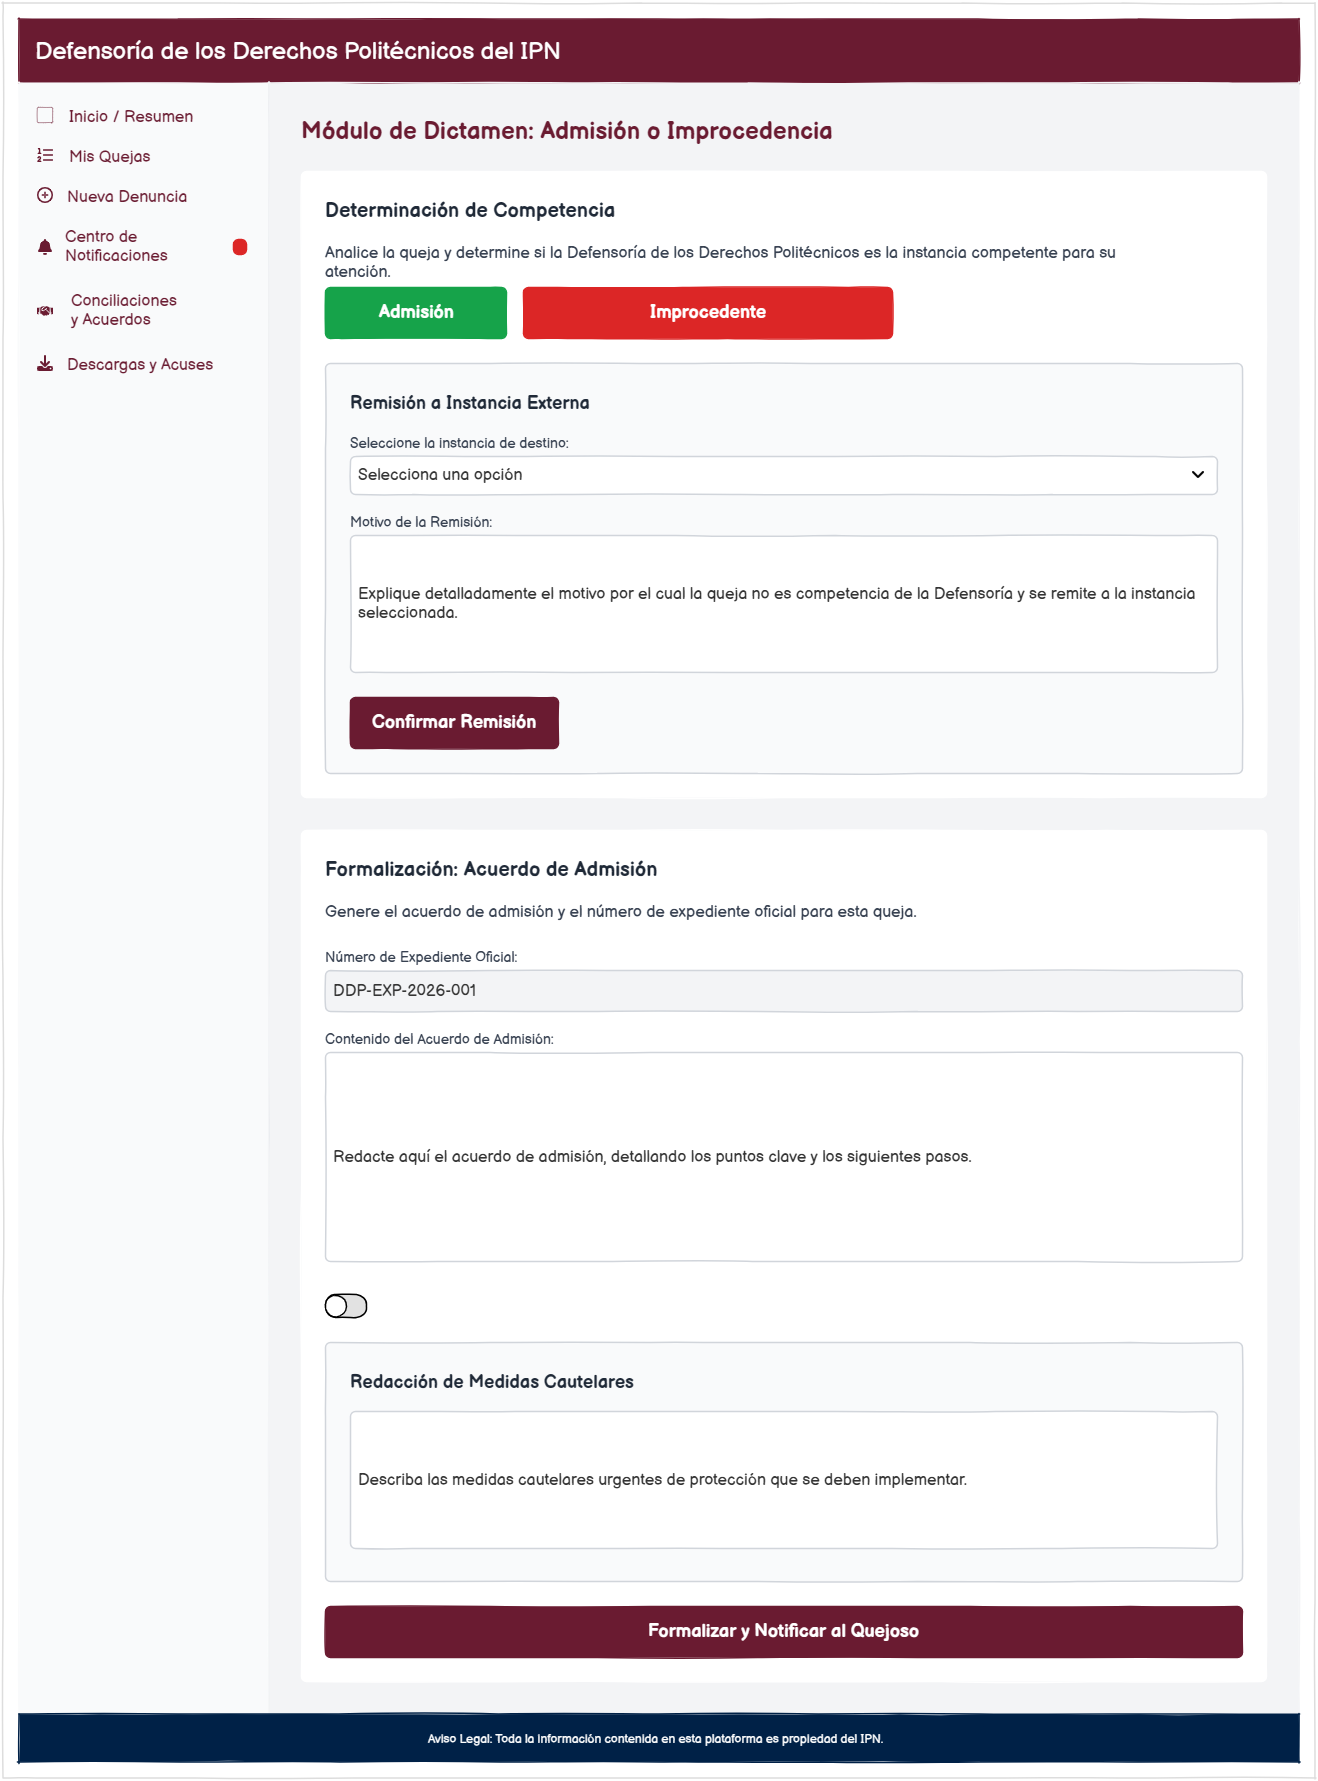
\includegraphics[width=0.65\textwidth]{imagenes/primercontacto/DictamenCompetencia}
\caption{MA-11: Módulo de dictamen de admisión o improcedencia.}
\label{fig:ma11_dictamen_competencia}
\end{figure}

\noindent \textbf{Descripción de la interfaz (MA-11):} \
Esta es la pantalla de resolución técnica donde se decide formalmente el curso legal de la queja presentada. El sistema ofrece botones de selección de alto contraste para definir la procedencia del caso, habilitando secciones específicas según la decisión tomada, ya sea para redactar los motivos legales de una improcedencia y su remisión externa, o para generar el número de expediente oficial en caso de admisión. La interfaz incluye también un control para la redacción de medidas cautelares urgentes en situaciones que requieran protección inmediata del quejoso. Una vez procesado el dictamen, el sistema formaliza el acto jurídico y prepara la notificación automática para el usuario.


\clearpage

% --- VISTA 12: FINALIZACIÓN Y NOTIFICACIÓN ---
\begin{figure}[h]
\centering
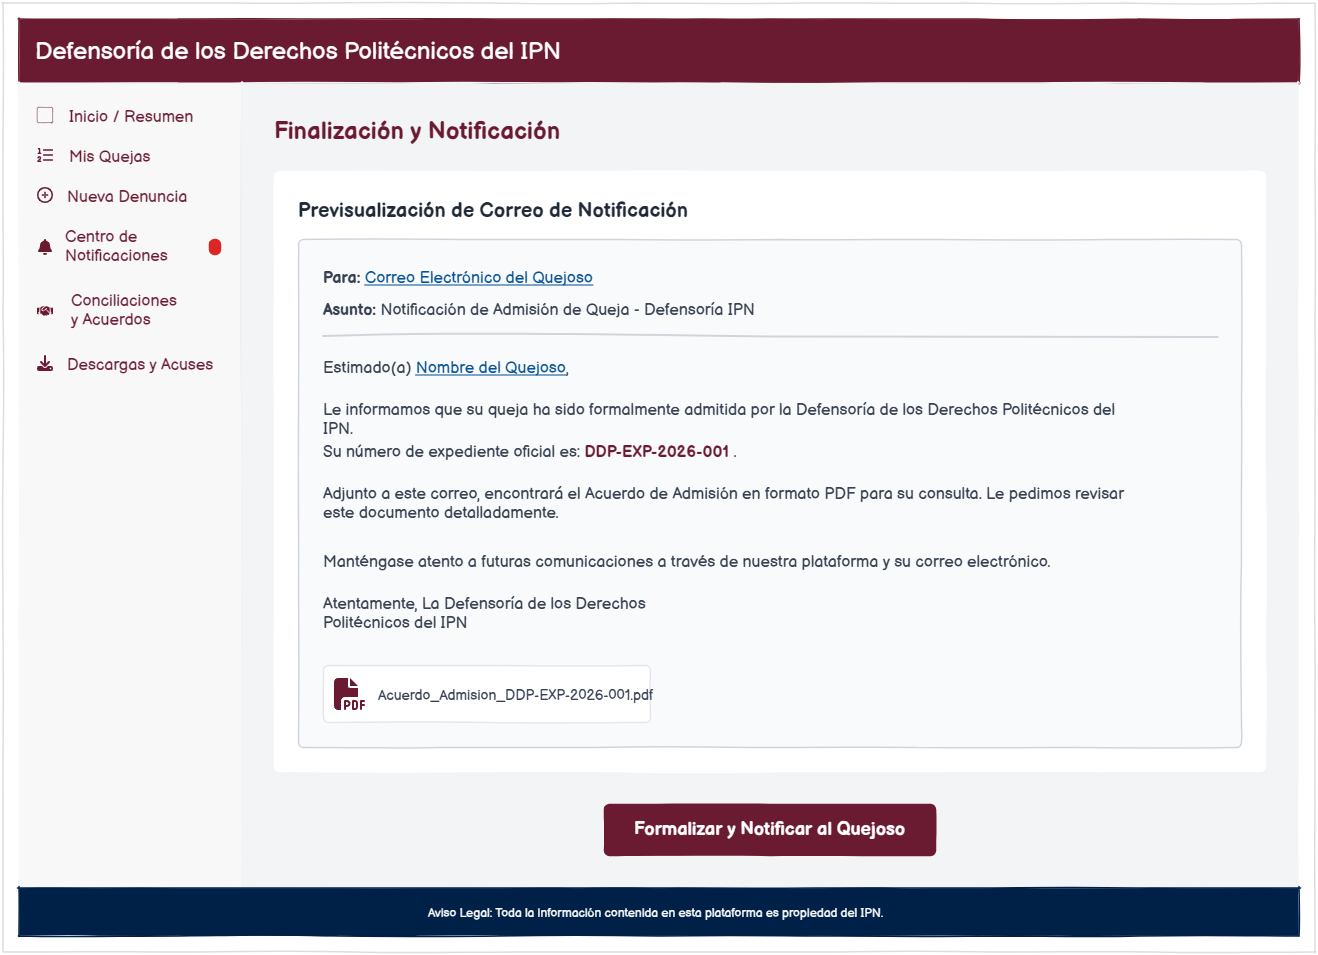
\includegraphics[width=0.65\textwidth]{imagenes/primercontacto/FormalizacionNotificacion.png}
\caption{MA-12: Interfaz de previsualización y notificación de admisión oficial.}
\label{fig:ma12_finalizacion_notificacion}
\end{figure}

\noindent \textbf{Descripción de la interfaz (MA-12):} \
Esta pantalla constituye el paso final del departamento de Primer Contacto antes de trasladar el expediente al área de instrucción en la Subdefensoría. Su propósito principal es garantizar la transparencia mediante una previsualización de la notificación oficial, permitiendo al analista verificar el cuerpo del correo electrónico y el número de expediente asignado. La interfaz muestra el archivo PDF del acuerdo de admisión vinculado y ofrece un botón de formalización que ejecuta simultáneamente el envío de la notificación y el cambio de estatus a "Admitida". De esta manera, se habilita el acceso al expediente para el siguiente departamento mientras el personal administrativo mantiene visibilidad sobre otras tareas pendientes en el entorno de gestión.

\end{appendices}